\section{\texorpdfstring{Maticovy popis grafu, det, kostry}{Maticovy popis grafu, det, kostry}}
	\vspace{5mm}
\large

%\begin{definition}
%Matice sousednosti grafu G
%\end{definition}

\begin{theorem}[Pocet sledu]
Pro kazdy graf G a každé přirozené číslo k obsahuje k-ta mocnina matice sousednosti A pocty sledu délky k mezi vrcholy grafu G, konkretně\\
$(A^k)_{a,b} = $ \# sledu délky k mezi a - b v G.
\end{theorem}
\begin{proof}
Indukci podle k.
\begin{enumerate}
	\item k = 0, sledy délky 0, neboli $ u - u $. Což odpovídá dle definice $ A^0 = I $.
	\item k = 1. Sled je pravě hrana.
	\item indukční krok:
	\[(A^{k+1})_{a,b} = (A^k * A)_{a,b} = \sum_{w \in V} (A^k)_{a,w} * A_{w,b} = \]
	na pozice $ (w,b) $ je 1 pokud existuje taková hrana, jinak 0. Proto
	\[ = \sum_{w, bw \in E} (A^k)_{a,w} = \]
	Dle I.P. se rovna poctu sledu délky k mezi $a - w$.
	Pak mezi vrcholy $ a - w $ existuje sled délky k.
	Rozdělíme sledy dle konečného vrcholu, který je soused $b$.
	Kazdy z těchto sledu jednoznačně prodloužíme na sled délky $(k+1)$ do vrcholu $b$. Z toho předchozí součet je pravě \# počet sledu délky $(k+1)$ mezi $ a - b $.
\end{enumerate}
\end{proof}

\begin{definition}
	$ L^{(n)}_G $ se dostane tak, ze vyškrtneme n-ty řádek a sloupec z Laplaceove matice.
\end{definition}
\begin{lemma}
\[ \forall w \subseteq E, |w| = n - 1: det((D^{(u)}_G)_w) = \twopartdef{0}{(V, w) \neq tree}{\pm 1}{ (V,w) = tree}  \]
\end{lemma}
\begin{proof}
		1) Nechť $w \subseteq E$ je kostra. Pak je stromem $\Rightarrow$ má list $v_1$. Přemístíme řádek odpovídající $v_1$ do prvního řádku. Nechť $e_1$ je hrana $v_1 - v_t$. Dáme ji do prvního sloupce.
		Pak na pozice (0,0) je $\pm 1$. Taky první řádek je $(\pm 1, 0, ... 0)$ protože vrchol je list.

	Odstraníme $v_1$, nechť $v_2$ je další list a $e_2$ jého hrana. Pak druhy řádek je $(??, \pm 1, 0, ... 0)$. Tak pokračujeme dal.

	Může se ale stát, ze další vrchol je $u$ který jsme zrovna odstranili. Použijeme tvrzeni, ze strom má aspoň 2 listy. Pak můžeme vzít nějaký další vrchol. Po ukončení přemisťovaní dostaneme $\pm 1$ na diagonále. Nad diagonálou same 0 $\Rightarrow det = \pm 1$. Přemístěním jsme měnili znamenko $det$. Ale $det^2 = 1$.

	2) Máme graf $w \subseteq E, |w| = |V| - 1$ který není strom $\Rightarrow$ není souvislý $\Rightarrow$ má aspoň 2 komponenty souvislosti. $V = V_1 \mathbin{\dot{\cup}} V_2$.
	BUNO $u \in V_2$. Pak z $V_1$ do $V_2$ nevede žádná hrana, část matice je 0. Pak součet řádku odpovídající $V_1, E(V_2)$ a $V_2, E(V_1)$ je 0 $\Rightarrow$ řádky jsou LZ a det je 0.

	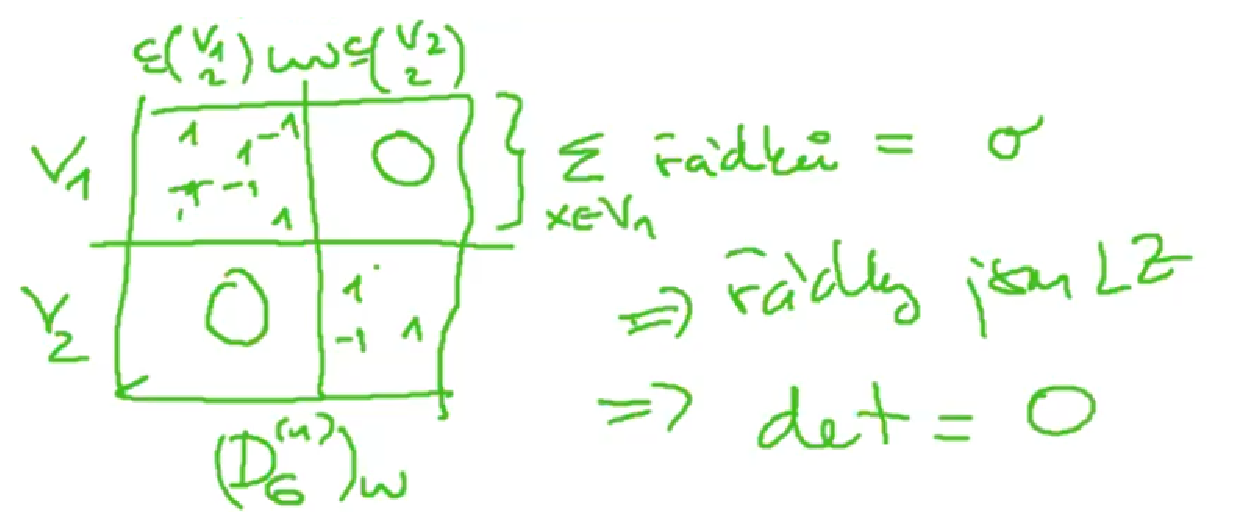
\includegraphics[scale=0.3]{kostra_lemma.eps}
\end{proof}

\begin{theorem}[Pocet koster]
	$ det(L^{(n)}_G) = $ \# koster grafu $G$.
\end{theorem}
\begin{proof}
	Vezmeme matice incidence $ I_G $ (jenom 2 jedničky ve sloupci, v řádku \# 1 je $deg(v)$), v každém její sloupci nahradíme jednu jedničku hodnotou $(-1)$. Výslednou matici označme $D_G$.

	$ I_G * I_G^T = $ skal. součin řádku i, j. Na diagonále $deg(v)$, mimo diag. 1 pro hrany, 0 - nehrany.

	Změníme pravě jednu 1ku ve každém sloupci na $-1$ (tím dostaneme orient. graf).
		\[ D_G * D_G^T = L_G \]
		Rovnost platí protože skalární součin stejného řádku dá $deg(v)$ jelikož $ -1 * -1 = 1 $. Pokud násobíme různé řádky, příslušné vrcholy nejsou spojené hranou - 0. Jinak mají pravě 1 společnou pozici a dostaneme $-1 * 1 = -1$.

	Pak $det(L^{(u)}_G)$ spočítáme jako $det(D^{(u)}_G * (D^{(u)}_G)^T)$

	Použijeme Cauchy-Benet vzoreček (det součiny obdelnikových matic)
	\[ det(A*B) = \sum _{\substack{ w \subseteq {1,2, ..., n} \\ |w| = k}} det A_w * det B^w \]
	Kde $ A_w $ jsou $n$ sloupců matice A, $ B^w $ - n řádku matice B.

	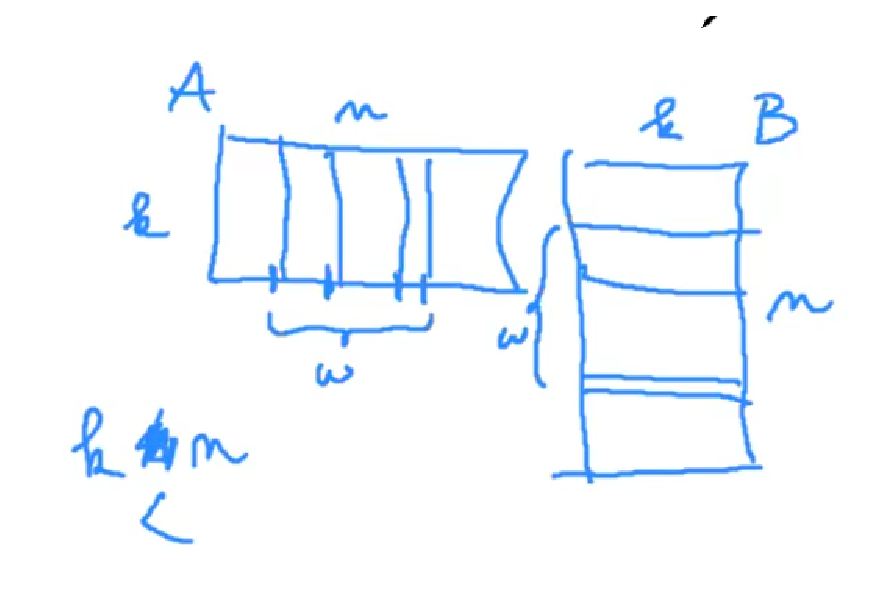
\includegraphics[scale=0.3]{cauchy-benet.eps}

	\[ det L^{(u)}_G = \sum_{\substack{w \subseteq E \\ |w| = n-1}} det(D^{(u)}_G) * (D^{(u)}_G)^{T} = \]
	Pro každou matici $ det A = det A^T $, pak
	\[ = \sum_{\substack{w \subseteq E \\ |w| = n-1}} det(D^{(u)}_G)^2 \]

	Kostra musí mít $(n-1)$ vrcholu; v det se díváme na všechny podmnožiny hran $|w| = n - 1$.
	Ptáme se jestli je strom. Proto suma nahoře je pravě
	\[ \sum_{\substack{w \\ (V,w) je \ kostra}} 1 \]
	Což je \# koster $G$

\end{proof}
